% Created 2016-08-17 Wed 14:38
\documentclass[tikz]{standalone}

\usepackage[utf8]{inputenc}
\usepackage[T1]{fontenc}
\usepackage{helvet}
\usepackage{../../templates/msc}

\renewcommand{\familydefault}{\sfdefault}

\tikzset{
every picture/.style={
line width=1pt
}}

\usepackage{tikz}
\author{Holger Karl}
\date{\today}
\title{}

\usetikzlibrary{decorations.pathmorphing}
\usetikzlibrary{calc}




\author{Holger Karl}
\date{\today}
\title{}

\author{Holger Karl}
\date{\today}
\title{}


\newcommand{\basescenario}{
\node[database] (db1) {S1}; 
\node[database] (db2) at (2,4) {S2}; 
\node[database] (db3) at (3,1) {S3}; 
\node[draw, dotted, inner sep=10pt, fit= (db1) (db2) (db3)] {}; 
\draw[dashed] (db1) -- (db2) -- (db3) -- (db1);

\node[below=1.5cm of db1] (w)  {Writer};
\node[bob, above=0cm of w] (wpic)  {};
\node[above left=of db2] (r1)  {Reader 1};
\node[alice, above=0cm of r1] {};
\node[right=of db3] (r2)  {Reader 2};
\node[alice, above=0cm of r2] {};
}

\newcommand{\basemessages}{
\draw [->] (wpic) to node [near start, right] {x=42!} (db1); 
\draw [->] (r1) to node [near start, auto]  {x=?} (db2); 
\draw [->] (r2) to node  [near start, auto] {x=?} (db3); 
}

\begin{document}


  \begin{tikzpicture}
    \basescenario \basemessages
  \end{tikzpicture}

\begin{tikzpicture}
  \basescenario \basemessages

  % partition
  \coordinate (tmp1) at ([shift={(0.75cm,1.5cm)}]db3); \coordinate
  (tmp2) at ([shift={(-1cm,1.cm)}]db3); \coordinate (tmp3) at
  ([shift={(-1.25cm,-1.2cm)}]db3); \coordinate (tmp4) at
  ([shift={(0.75cm,-1.4cm)}]db3);

  \draw [red, decorate, decoration={snake}] (tmp1) -- (tmp2) -- (tmp3)
  -- (tmp4);
\end{tikzpicture}


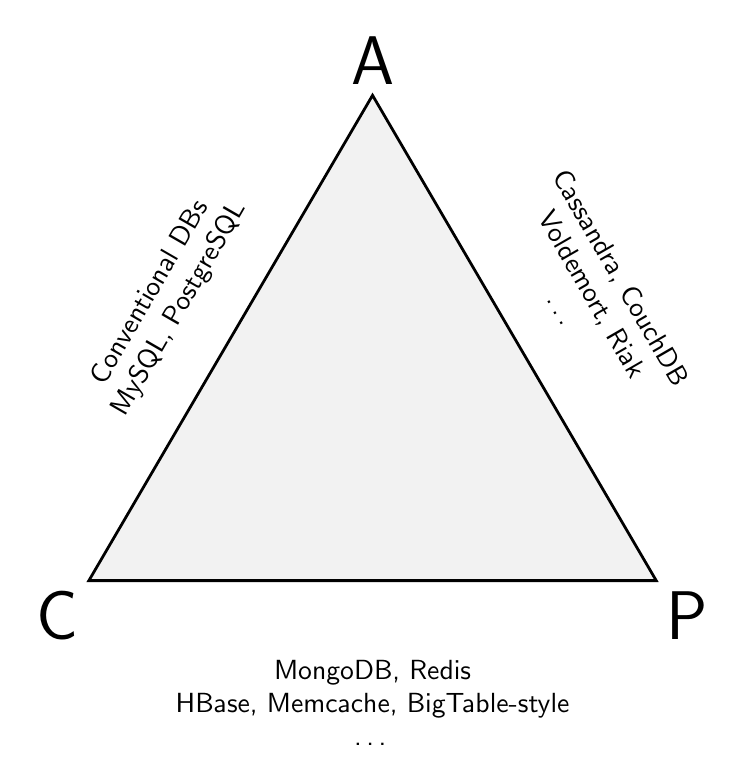
\begin{tikzpicture}
  % CAP landscape 
  \node at (-4, 0) (C)  {\Huge C}; 
  \node at (+4, 0) (P)  {\Huge P}; 
  \node at (0, 4*1.76) (A)  {\Huge A}; 

  \draw [fill=gray!10] (C.north east) -- (A.south) -- (P.north west) -- cycle;

  \node [rotate=60,anchor=south,align=center] at ($ (C.north)!0.5!(A.west)$) {Conventional DBs\\MySQL, PostgreSQL};

  \node [align=center,anchor=south,rotate=-60] at  ($ (P.north)!0.5!(A.east)$) {Cassandra, CouchDB\\Voldemort, Riak\\\ldots};

  \node [align=center,anchor=north] at  ($ (P.south)!0.5!(C.south)$) {MongoDB, Redis\\HBase, Memcache, BigTable-style\\\ldots};

\end{tikzpicture}

\end{document}